In graph theory, the \textit{tournoi} is an oriented clique. This currently inscribes a sequence in a temporal configuration, where the \textit{fanaux} -- by nature timeless -- will then create links oriented in the form of cliques, in other words \textit{tournoi}.

\begin{figure}[htbp]
    \centering
    \begin{minipage}{0.5\textwidth}
        \centering
                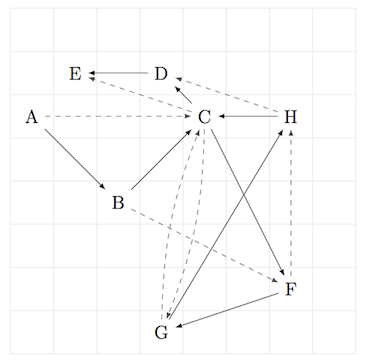
\includegraphics[width=0.9\textwidth]{2402} % second figure itself
        \caption{Example of application of \textit{tournois} \citep{bg1}, op. cit., page 117.}
        \label{fig:trn2}
            \end{minipage}\hfill
    \begin{minipage}{0.45\textwidth}
        \centering
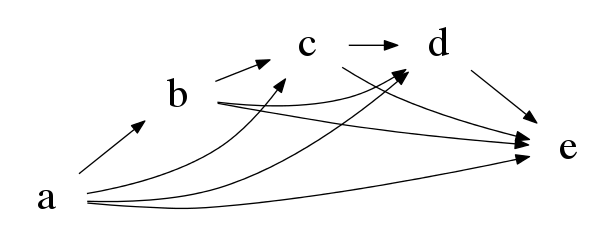
\includegraphics[width=0.9\textwidth]{2401} % first figure itself
        \caption{Here is an example of a 5 order \textit{tournoi}. This one corresponds to the followings arcs: ((a b) (a c) (a d) (a e) (b c) (b d) (b e) (c d) (c e) (d e)) and which will be translated simply by: (a b c d e).}
      \label{fig:trn1}

    \end{minipage}
\end{figure}

\bigskip

To illustrate an application of \textit{tournois}, the figure \ref{fig:trn2} shows a directed graph, in which we seek to restore the path A-B-C-F-G-H-C-D-E unambiguously -- represented with full arrows. Each node symbolizes an \textit{infon}. At first, the problem lies at node C, where two options are possible, namely F or D. A \textit{tournoi} of order 3 solves this problem, covering 2 successive nodes -- represented by dashed arrows --, anticipating thus the path from C to F signaled by the arrows from B to F when we come from B.

\bigskip

Thus, the temporal overlap depends on the order\footnote{In the graph theory, the order is the number of nodes interconnected. For both the \textit{tournoi} and the clique as a complete graph, the order allows to determinate the number of edges needed such as for a graph of order $n$, the number of edges is equal to $n(n-1)/2$ -- see example figure \ref{fig:trn1}.} of the \textit{tournoi}, i.e. $n-1$ and will determine the anticipation capacity of the network.